\documentclass[a4paper]{article}

%\usepackage{ctex}
\usepackage{fancyhdr}
% \usepackage{extramarks}
\usepackage{cite}
\usepackage{color}
\usepackage{float}
\usepackage{amsmath}
\usepackage{amsthm}
\usepackage{setspace}
\usepackage{amsmath}
\usepackage{amssymb}
\usepackage{cmap}
\usepackage{graphicx}
\usepackage{geometry}
\usepackage{hyperref}
\usepackage{indentfirst}
\usepackage{makecell}
\usepackage{mathrsfs}
\usepackage{multirow}
\usepackage{enumerate}
\usepackage{bm}
\usepackage{algpseudocode}
\usepackage{algorithm}
\usepackage{tikz}
\usepackage{subcaption}
\usetikzlibrary{automata,positioning,topaths}
%\usepackage{xeCJK}
%\usepackage{minted}
\title{
	\vspace{2in}
	\textbf{\courseName} \\
	\textbf{\homeworkID} \\
	\semester
	\vspace{3in}
}
\author{
	\textbf{\authorName} \\
	Student ID: \authorID
}
\date{}

\topmargin=-0.45in
\evensidemargin=0in
\oddsidemargin=0in
\textwidth=6.5in
\textheight=9.0in
\headsep=0.25in

\linespread{1.2}

\pagestyle{fancy}
\lhead{\authorName}
\chead{\courseName}
\rhead{Problem \arabic{chapterCounter}.\arabic{problemCounter}}
\cfoot{\thepage}

\newcounter{chapterCounter}
\newcounter{problemCounter}
\newcounter{partCounter}

\newenvironment{problem}[2]{
	\setcounter{chapterCounter}{#1}
	\setcounter{problemCounter}{#2}
	\section*{Problem \arabic{chapterCounter}.\arabic{problemCounter}}
	\setcounter{partCounter}{1}
}{}
\newenvironment{subproblem}[0]{
	\subsection*{Part \Alph{partCounter}}
	\stepcounter{partCounter}
}{}

\newtheorem{theorem}{Theorem}%[section]
\newtheorem{proposition}[theorem]{Proposition}
\newtheorem{lemma}[theorem]{Lemma}
\newtheorem{corollary}[theorem]{Corollary}
\newtheorem{definition}[theorem]{Definition}

\newcommand{\solution}{\paragraph{Solution}}
\newcommand{\upperbound}[1]{O\left(#1\right)}
\newcommand{\lowerbound}[1]{\Omega\left(#1\right)}
\newcommand{\exactbound}[1]{\Theta\left(#1\right)}

\newcommand{\Z}{\mathbb{Z}}
\newcommand{\R}{\mathbb{R}}
\newcommand{\Q}{\mathbb{Q}}
\newcommand{\N}{\mathbb{N}}
\newcommand{\downcast}[1]{\lfloor#1\rfloor}
\newcommand{\upcast}[1]{\lceil#1\rceil}
\newcommand{\courseName}{Deep Learning and Application}
\newcommand{\homeworkID}{Final Project}
\newcommand{\authorName}{Tianyao Chen, Runzhe Yang, Xingyuan Sun}
\newcommand{\authorID}{5140309566, 5140309562, 5140309561}
\newcommand{\semester}{2016-2017 Fall}
\begin{document}



\maketitle
\pagebreak

\section{Introduction}

In this report, we proposed some methods for processing data in tone classification problem, used several deep neural networks structure, did some experiments, and compared their performance and time consumptions among three popular deep learning toolkits: {\bf Torch}, {\bf Theano} and {\bf Tensorflow}.

The data set that our teaching assistances gave us has only $400$ data for training. This is a number that is not so sufficient for very large or very deep network to train. Since then, we can only use some small networks. But the data is not so regular that small networks can not separate the original data. This situation forces us to find some way to preprocess our data, then to feed the preprocessed data into the networks.

\section{Data Preprocessing}

Our prior knowledge tells us that the tone recognition task only requires pitch contour information, which can be expressed by fundamental frequency. Fortunately, the feature \texttt{f0} as well as \texttt{engy} feature have already given to us. But it does not mean we can use the \texttt{f0} feature directly for three reasons: 1) there are some noise and redundant information in the raw \texttt{f0} feature, which would be great distraction; 2) there numerical values of \texttt{f0} feature varies in a large range so that it will increase difficulties when training; 3) the sequences of features are not of the same length so that it is not suitable for a wide range of models. Therefore, we can not circumvent data preprocessing part. In this section, we will introduce a pipeline of data preprocessing for normalization, removing redundant information, smoothing and denoising data and finally expanding to the same length. Experiments show that data preprocessing can influence performance of models significantly.
\subsection{Mel Scale}
We first convert the foundational frequency (\texttt{f0}) in the mel-scale. The reason we do that is the Mel frequency is much closer the non-linear sensing measurement of human listeners. We use a popular version\footnote{\url{https://en.wikipedia.org/wiki/Mel-frequency_cepstrum}} of mel-scale formula as
	\[\mathtt{Mel}(f) = 2595\log_{10}(1+f/ 700).\]
	
However, the frequencies in mel-scale are not very robust in the presence of additive noise, and so it is common to normalize them in speech recognition systems to lessen the influence of noise.
\subsection{Standardization}
When normalizing data, we only divide its standard derivation but do not subtract its mean, since there are some zeros in the data sequence. Besides, we conduct two types of standardization. One is called \textbf{local standardization}, in which divide the \texttt{std} of a certain feature it self, to avoid some data varies in a huge range. The other is to divide the \texttt{std} of the whole data set for easier training, called \textbf{global standardization}. We do the local standardization first, then do global standardization, for both \texttt{f0} and \texttt{engy}.
\subsection{Removing Redundancy}
As we observe in the training data, there some redundancies in the \texttt{f0} features: Although the \texttt{engy} is very low (even is zero), the \texttt{f0} is still very high and behaves strangely. We think this part of \texttt{f0} is redundant because even human listeners cannot recognize a tone in very low volume. Further, this part of \texttt{f0} is more likely from environments instead of human speaker because of low corresponding \texttt{engy}. Hence, in data preprocessing, we discard the redundancies of \texttt{f0} such that corresponding $\mathtt{standardized(engy)} < 1.0$. 

We only keep the non-zero part of \texttt{f0} after processing as the output of this stage. This part of data still contains some noise. So in the next step, we are going to try to denoise the \texttt{f0} feature.

\subsection{Smoothing}
The extracted \texttt{f0} alway has some obvious double, half or random error point. We need to do further smoothing for offering better feature to the tone recognizer. Typically, we can use some approaches such as linear interpolation, moving average to make the frequencies varies smoothly. But those method cannot deal with the case that data containing continuous random error points which is quite common in our dataset. We use a search-based algorithm
%	\cite{tone:2000}
	to smooth the frequency data. In that paper, the author used this algorithm to decrease the recognition error rate by $40\%$. 
	
We search from a smooth beginning of \texttt{f0} data, and adjust each data point in order. Let $f_1, f_2, \dots, f_{N}$ be the frequencies of $N$ continues frames. When we deal with the $i$-th data point $f_i$ we first deal with the case of double of half frequency. If 
\[ |f_i / 2 - f_{i-1}| < C_1 \text{, then we let } f'_i = f_i / 2;\]
else if 
\[ |2 \cdot f_i- f_{i-1}| < C_1 \text{, then we let } f'_i = 2 \cdot f_i.\]
Then for random error point (noise), if
\[|f_i - f_{i - 1}| > C_1 \text{ and } |f_{i + 1} - f_{i - 1}| > C_2,\text{, then we let } f'_i = 2 \cdot f_{i- 1} - f_{i - 2}. \]
else if
\[|f_i - f_{i - 1}| > C_1 \text{ and } |f_{i + 1} - f_{i - 1}| \leq C_2,\text{, then we let } f'_i = 0.5 \cdot f_{i + 1} + f_{i - 1}. \]
otherwise, the data point is not an error point, we simply keep $f'_i = f_i$. When we deal with the frequency $f_{i+1}$ of next frame, we substitute $f_{i}$ with $f'_i$. By observing the smoothed \texttt{f0} in training set, we adopt $C_1 = 0.32$ and $C_2 = 0.67$ in our experimental settings.

The process above is good for the level tone, the rising tone and the falling tone, but for the falling-rising tone, it will change the shape of data curve. To solve this, we can do the same process as above but from the $N$-th frame to the first frame.

Finally, we use moving average with a window of size $5$ frames to further smooth data. Moving averaging can not only remove the random error points but also keep the stepped transition between two smooth periods.

\subsection{Data Expansion}
By here, we have already get a denoised \texttt{f0}. But they are not of the same length and it is annoying if we want to use them to train a normal fully connected neural network or convolutional neural network. We come up with three ways to expand the data into the same length. Three ways corresponding three different datasets. They are
\begin{enumerate}
\item data.shift

	This dataset is made by shift the beginning of smoothed \texttt{f0} feature to its first non-zero element. Then we pad $0$s at the end of the data to make its length be $128$.

	The dataset is saved in file ``shared data/data\_shift.json''.
\item data.linear

	In this dataset, we use expand the dataset by linear interpretation. Suppose the smoothed \texttt{f0} feature has $N$ frames, we want to expand it to $N'$ frame data, then the missing data $f'_j$ between original smoothed \texttt{f0} data $f_{i}$ and $f_{i+1}$ should be
	\[ f'_{j} =  (f_{i+1} - f_{i})\left(\frac{(j - 1)(N - 1)}{N' - 1}- i + 1\right) + f_i\]
	and $f'_{1} = f_1$, $f'_{N'} = f_{N}$ should hold as boundary condition.

	The dataset is saved in file ``shared data/data\_linear.json''.

\item data.quad
	
	Another way is using a quadratic function to fit the curve of smoothed \texttt{f0} feature. If the fit curve obtained by least square method is $g(x) = a + bx + cx^2$, then the missing data $f'_j$ between original smoothed \texttt{f0} data $f_{i}$ and $f_{i+1}$ should be scaled as
\[ f'_{j} =  g[(j - 1) (N - 1) / (N' - 1)  + 1]\]

	The dataset is saved in file ``shared data/data\_quad.json''.

\end{enumerate}

\begin{figure}[H]
	\centering
	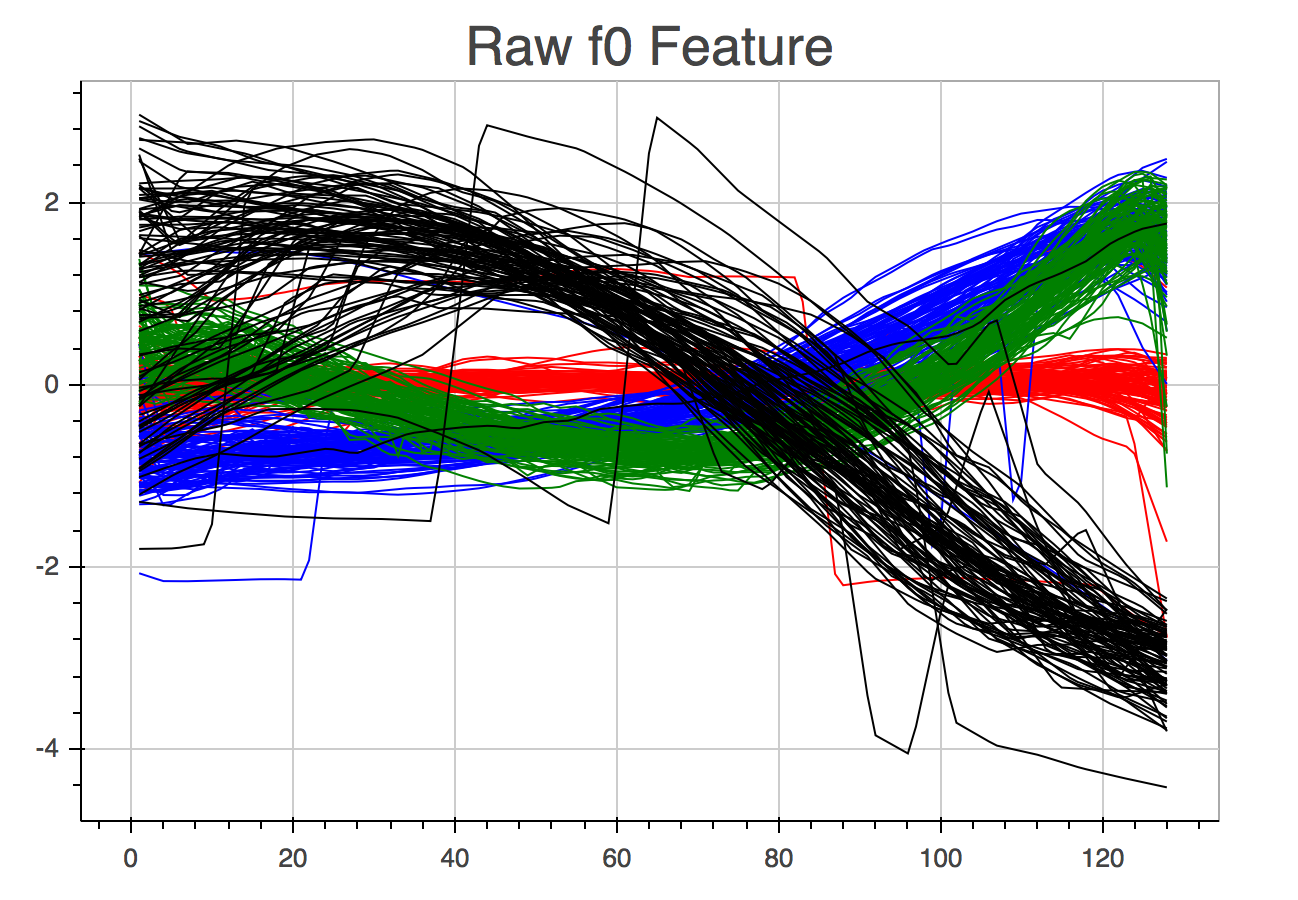
\includegraphics[width = 0.4\textwidth]{figs/f0}
	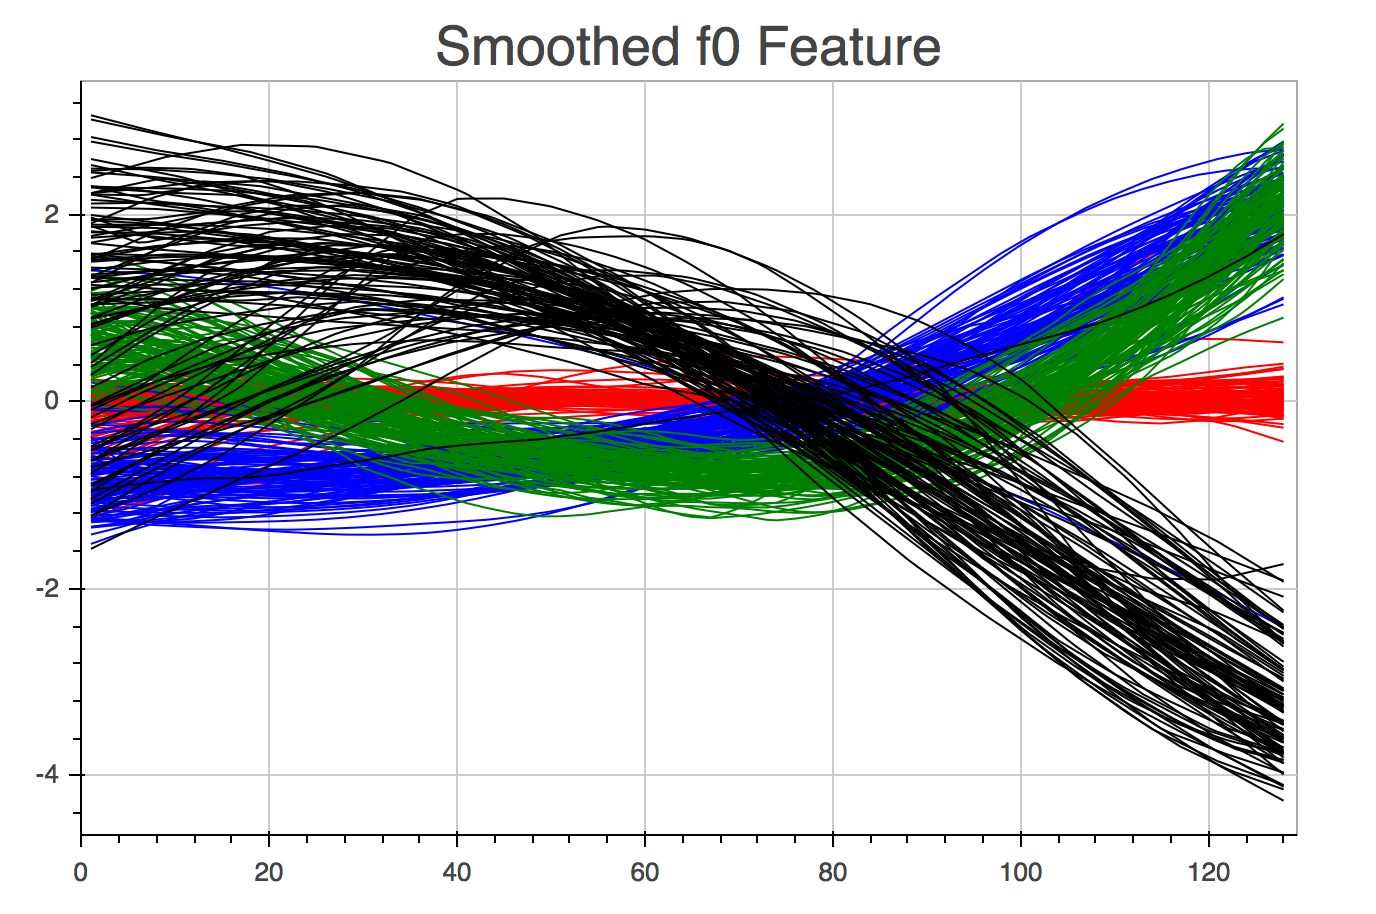
\includegraphics[width = 0.4\textwidth]{figs/Sf0}
	\caption{Left: the \texttt{f0} features in the training set without smoothing; Right: the \texttt{f0} features in the training set after smoothing; Both are expanded to the length of 128 frames by linear interpolation.}
\end{figure}

\subsection{Centralization}
For \texttt{data.linear} and \texttt{data.quad} we subtract their mean in the last step. The reason we do not apply centralization on  \texttt{data.quad} is we pad zero at the end of the data and do not want that part contains any information. Up to now, we have finish the data preprocessing part.

\subsection{Other Approaches}
Admittedly, rule-based data processing always has some drawbacks and cannot denoising very well. Therefore we also tried some other approaches using deep learning technique. One of them is denoising autoencoder (DAE). This approach can provide us a robust feature extraction and generating more data so that we can do  {\bf data augmentation}. However in experiment we found that the noise of \texttt{f0} is not Gaussian and adding white noise cannot improve its robustness. We discard this way.

\section{Models}

We tested two models on the datasets we have made.
\begin{enumerate}
\item pure.fc

	This model has just one fully connected layer. Suppose our input is just $1$-dimensional raw vector $x$, with weight matrix $W$ and bias vector $b$, the scores for the four tones are
	\[
		\text{score} = x \cdot W + b
	\]
	We use softmax loss and l$2$-norm regularization.

\item cnn.fc

	This model has one convolution layer with a 2-strided max-pooling layer followed by one fully connected layer.

\end{enumerate}

\section{Experiments}

We tried each model on each dataset, implemented by each framework.

\subsection{Hyperparameters}

\begin{figure}[H]
\centering
\begin{tabular}{|r|c|c|c|}
\hline
 & value \\
\hline
regularization strength & $0.01$ \\
\hline
batch size & $10$ \\
\hline
optimizer & SGD \\
\hline
learning rate & $3\times10^{-5}$\\
\hline
learning rate decay & N/A \\
\hline
number of epochs & $2000$ \\
\hline
\end{tabular}
\caption{Hyperparameters settings for ``pure.fc'' model.}
\end{figure}

\begin{figure}[H]
\centering
\begin{tabular}{|r|c|c|c|}
\hline
 & value \\
\hline
filter size & $3$ \\
\hline
number of channels & $64$ \\
\hline
regularization strength & $0.002$ \\
\hline
batch size & $10$ \\
\hline
optimizer & SGD \\
\hline
learning rate & $1\times10^{-4}$\\
\hline
learning rate decay & N/A \\
\hline
number of epochs & $400$ \\
\hline
\end{tabular}
\caption{Hyperparameters settings for ``cnn.fc'' model.}
\end{figure}

\subsection{Experiments result}

Now we show the performance and time consumption.

\begin{figure}[H]
\centering
\begin{tabular}{|r|r|c|c|c|}
\hline
 & & data.shift & data.linear & data.quad \\
\hline
pure.fc & training set accuracy & \\
 & test set accuracy & \\
 & test\_new set accuracy & \\
 & time & \\
\hline
cnn.fc & training set accuracy & \\
 & test set accuracy & \\
 & test\_new set accuracy & \\
 & time & \\
\hline
\end{tabular}
\caption{Performance and time consumption on Torch.}
\end{figure}

\begin{figure}[H]
\centering
\begin{tabular}{|r|r|c|c|c|}
\hline
 & & data.shift & data.linear & data.quad \\
\hline
pure.fc & training set accuracy & \\
 & test set accuracy & \\
 & test\_new set accuracy & \\
 & time & \\
\hline
cnn.fc & training set accuracy & \\
 & test set accuracy & \\
 & test\_new set accuracy & \\
 & time & \\
\hline
\end{tabular}
\caption{Performance and time consumption on Theano.}
\end{figure}

\begin{figure}[H]
\centering
\begin{tabular}{|r|r|c|c|c|}
\hline
 & & data.shift & data.linear & data.quad \\
\hline
pure.fc & training set accuracy & $85.25\%$ & $91.00\%$ & $92.75\%$ \\
 & test set accuracy & $80.00\%$ & $100.00\%$ & $100.00\%$ \\
 & test\_new set accuracy & $55.26\%$ & $92.54\%$ & $92.98\%$ \\
 & time & $36.30$s & $35.92$s & $34.87$s \\
\hline
cnn.fc & training set accuracy & $84.75\%$ & $93.25\%$ & $90.25\%$ \\
 & test set accuracy & $70.00\%$ & $90.00\%$ & $95.00\%$ \\
 & test\_new set accuracy & $54.82\%$ & $90.35\%$ & $94.74\%$ \\
 & time & $30.18$s & $34.44$s & $37.21$s \\
\hline
\end{tabular}
\caption{Performance and time consumption on Tensorflow.}
\end{figure}

\section{Conclusion}

\section{References}
\bibliography{main}

\bibliographystyle{main}

\end{document}